\documentclass[Royal,times,sageh]{sagej}

\usepackage{moreverb,url,natbib, multirow, tabularx}
\usepackage[colorlinks,bookmarksopen,bookmarksnumbered,citecolor=red,urlcolor=red]{hyperref}



% tightlist command for lists without linebreak
\providecommand{\tightlist}{%
  \setlength{\itemsep}{0pt}\setlength{\parskip}{0pt}}





\begin{document}


\setcitestyle{aysep={,}}

\title{A demonstration of the \LaTeX class file for Statistical Methods
in Medical Research with Rmarkdown}

\runninghead{Uthor \emph{et al}.}

\author{A. Uthor*\affilnum{1,2}, O. Tro\affilnum{2}, O.
Vriga\affilnum{3}}

\affiliation{\affilnum{1}{Department of Incredible Research, University
A, City A, Country A}\\\affilnum{2}{Department of Applied Things,
University B, City B, Country B}\\\affilnum{3}{Very Important Stuff
Committee, Institute C, City C, Country C}}

\corrauth{Corresponding author name, This is sample corresponding
address.}

\email{\href{mailto:correspondingauthor@protonmail.com}{\nolinkurl{correspondingauthor@protonmail.com}}}

\begin{abstract}
Lorem ipsum dolor sit amet, consectetur adipiscing elit. Aenean ut elit
odio. Donec fermentum tellus neque, vitae fringilla orci pretium vitae.
Fusce maximus finibus facilisis. Donec ut ullamcorper turpis. Donec ut
porta ipsum. Nullam cursus mauris a sapien ornare pulvinar. Aenean
malesuada molestie erat quis mattis. Praesent scelerisque posuere
faucibus. Praesent nunc nulla, ullamcorper ut ullamcorper sed, molestie
ut est. Donec consequat libero nisi, non semper velit vulputate et.
Quisque eleifend tincidunt ligula, bibendum finibus massa cursus eget.
Curabitur aliquet vehicula quam non pulvinar. Aliquam facilisis tortor
nec purus finibus, sit amet elementum eros sodales. Ut porta porttitor
vestibulum. Integer molestie, leo ut maximus aliquam, velit dui iaculis
nibh, eget hendrerit purus risus sit amet dolor. Sed sed tincidunt ex.
Curabitur imperdiet egestas tellus in iaculis. Maecenas ante neque,
pretium vel nisl at, lobortis lacinia neque. In gravida elit vel
volutpat imperdiet. Sed ut nulla arcu. Proin blandit interdum ex sit
amet laoreet. Phasellus efficitur, sem hendrerit mattis dapibus, nunc
tellus ornare nisi, nec eleifend enim nibh ac ipsum. Aenean tincidunt
nisl sit amet facilisis faucibus. Donec odio erat, bibendum eu imperdiet
sed, gravida luctus turpis.
\end{abstract}

\keywords{Class file; \LaTeX; SMMR; Rmarkdown;}

\maketitle

\hypertarget{the-article-header-information}{%
\section{The Article Header
Information}\label{the-article-header-information}}

YAML header:

\begin{verbatim}
output:
  rticles::sim_article:
    keep_tex: TRUE
\end{verbatim}

Configure the YAML header including the following elements:

\begin{itemize}
\item
  \texttt{title}: Title
\item
  \texttt{runninghead}: Author last names, use \emph{et al.} if there
  are three or more authors.
\item
  \texttt{author}: List of author(s) containing \texttt{name} and
  \texttt{num}
\item
  \texttt{corrauth}: Corresponding author's name and address.
\item
  \texttt{email}: Correspondence email
\item
  \texttt{abstract}: Limited to 200 words
\item
  \texttt{keywords}: Keywords for the article
\item
  \texttt{bibliography}: BibTeX \texttt{.bib} file
\item
  \texttt{bibliographystyle}: sageh or sagev
\item
  \texttt{classoption}: options of the \texttt{sagej} class
\end{itemize}

\hypertarget{remarks}{%
\subsection{Remarks}\label{remarks}}

\begin{enumerate}
\def\labelenumi{\arabic{enumi}.}
\setcounter{enumi}{1}
\item
  \texttt{bibliographystyle}
\item
  \texttt{classoption}
\item
  Keywords are separated by commas.
\end{enumerate}

\hypertarget{the-body-of-the-article}{%
\section{The Body of the Article}\label{the-body-of-the-article}}

\hypertarget{mathematics}{%
\subsection{Mathematics}\label{mathematics}}

Use mathematics in Rmarkdown as usual.

\hypertarget{figures-and-tables}{%
\subsection{Figures and Tables}\label{figures-and-tables}}

Figures are supported from R code:

\begin{verbatim}
x = rnorm(10)
y = rnorm(10)
plot(x, y)
\end{verbatim}

\begin{figure}
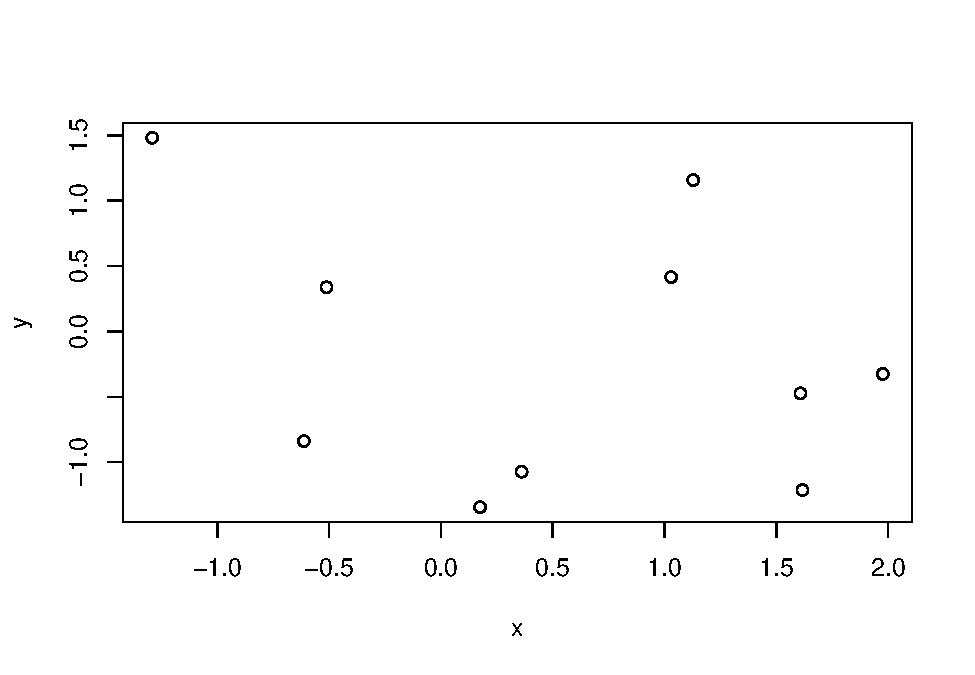
\includegraphics[width=1\linewidth]{Untitled_files/figure-latex/plot-ref-1} \caption{Fancy Caption\label{fig:plot}}\label{fig:plot-ref}
\end{figure}

\ldots and can be referenced (Figure \ref{fig:plot}) by including the
\texttt{\textbackslash{}\textbackslash{}label\{\}} tag in the
\texttt{fig.cap} attribute of the R chunk:
\texttt{fig.cap\ =\ "Fancy\ Caption\textbackslash{}\textbackslash{}label\{fig:plot\}"}.
It is a quirky hack at the moment, see
\href{https://github.com/yihui/knitr/issues/323}{here}.

Analogously, use Rmarkdown to produce tables as usual:

\begin{verbatim}
if (!require("xtable")) install.packages("xtable")
\end{verbatim}

\begin{verbatim}
## Loading required package: xtable
\end{verbatim}

\begin{verbatim}
xt <- xtable(head(cars), caption = "A table", label = "tab:table")
print(xt, comment = FALSE)
\end{verbatim}

\begin{table}[ht]
\centering
\begin{tabular}{rrr}
  \hline
 & speed & dist \\ 
  \hline
1 & 4.00 & 2.00 \\ 
  2 & 4.00 & 10.00 \\ 
  3 & 7.00 & 4.00 \\ 
  4 & 7.00 & 22.00 \\ 
  5 & 8.00 & 16.00 \\ 
  6 & 9.00 & 10.00 \\ 
   \hline
\end{tabular}
\caption{A table} 
\label{tab:table}
\end{table}

Referenced via \ref{tab:table}. You can also use the YAML option
\texttt{header-includes} to includes custom \LaTeX packages for tables
(keep in mind that \texttt{pandoc} uses \texttt{longtables} by default,
and it is hardcoded; some things may require including the package
\texttt{longtable}). E.g., using \texttt{ctable}:

\begin{verbatim}
header-includes:
- \usepackage{ctable}
\end{verbatim}

Then, just write straight-up \LaTeX code and reference is as usual
(\texttt{\textbackslash{}ref\{tab:ctable\}}):

\begin{verbatim}
\ctable[cap = {Short caption},
        caption = {A caption for this table.},
        label={tab:ctable},]
        {cc}
        {
        \tnote[$\ast$]{Footnote 1}
        \tnote[$\dagger$]{Other footnote}
        \tnote[b]{Mistakes are possible.}
        }{
        \FL
        COL 1\tmark[a] & COL 2\tmark[$\ast$]
        \ML
        6.92\tmark[$\dagger$] & 0.09781 \\
        6.93\tmark[$\dagger$] & 0.09901 \\
        97 & 2000
        \LL
}
\end{verbatim}

It is also possible to set the \texttt{YAML} option
\texttt{longtable:\ true} and use markdown tables (or the
\texttt{knitr::kable} function): \texttt{knitr::kable(head(cars))}
produces the same table as the \texttt{xtable} example presented before.

\hypertarget{cross-referencing}{%
\subsection{Cross-referencing}\label{cross-referencing}}

The use of the Rmarkdown equivalent of the \LaTeX cross-reference system
for figures, tables, equations, etc., is encouraged (using
\texttt{{[}@\textless{}name\textgreater{}{]}}, equivalent of
\texttt{\textbackslash{}ref\{\textless{}name\textgreater{}\}} and
\texttt{\textbackslash{}label\{\textless{}name\textgreater{}\}}). That
works well for citations in Rmarkdown, not so well for figures and
tables. In that case, it is possible to revert to standard
\LaTeX syntax.

\hypertarget{double-spacing}{%
\subsection{Double Spacing}\label{double-spacing}}

If you need to double space your document for submission please use the
\texttt{doublespace} option in the header.

\hypertarget{bibliography}{%
\section{Bibliography}\label{bibliography}}

Link a \texttt{.bib} document via the YAML header, and bibliography will
be printed at the very end (as usual). The default bibliography style is
provided by Wiley as in \texttt{WileyNJD-AMA.bst}, do not delete that
file.

Use the Rmarkdown equivalent of the \LaTeX citation system using
\texttt{{[}@\textless{}name\textgreater{}{]}}. Example:
\citep{Taylor1937}, \citep{Knupp1999, Kamm2000}.

To include all citation from the \texttt{.bib} file, add
\texttt{\textbackslash{}nocite\{*\}} before the end of the document.

\hypertarget{further-information}{%
\section{Further information}\label{further-information}}

All \LaTeX enviroments supported by the main template are supported here
as well; see the \texttt{.tex} sample file
\href{http://onlinelibrary.wiley.com/journal/10.1002/(ISSN)1097-0258/homepage/la_tex_class_file.htm}{here}
for more details and example.

\bibliographystyle{sageh}
\bibliography{bibfile}


\end{document}
